% PVLDB Vol. 20 (VLDB 2027) submission. Template: https://github.com/cwida/pvldbstyle (acmart sigconf, nonacm).
\documentclass[sigconf, nonacm]{acmart}

%% The following content must be adapted for the final version
% paper-specific
\newcommand\vldbdoi{XX.XX/XXX.XX}
\newcommand\vldbpages{XXX-XXX}
% issue-specific
\newcommand\vldbvolume{20}
\newcommand\vldbissue{1}
\newcommand\vldbyear{2027}
% should be fine as it is
\newcommand\vldbauthors{\authors}
\newcommand\vldbtitle{\shorttitle}
% leave empty if no availability url should be set
\newcommand\vldbavailabilityurl{}
% whether page numbers should be shown or not, use 'plain' for review versions, 'empty' for camera ready
\newcommand\vldbpagestyle{plain}

\usepackage{booktabs}
\usepackage{tikz}
\usetikzlibrary{positioning,arrows.meta,calc,fit}
\definecolor{opblue}{HTML}{2A78D6}
\definecolor{ixorange}{HTML}{EB6834}
\definecolor{engine}{HTML}{898781}
\usepackage{xspace}
\usepackage{listings}
\usepackage{xcolor}

\newcommand{\duckpgq}{DuckPGQ\xspace}
\newcommand{\duckdb}{DuckDB\xspace}
\newcommand{\sqlpgq}{SQL/PGQ\xspace}
\newcommand{\msbfs}{MS-BFS\xspace}
\newcommand{\todo}[1]{\textcolor{red}{[TODO: #1]}}
\newcommand{\cn}{\textcolor{red}{[cite]}\xspace}

\lstset{basicstyle=\ttfamily\small, breaklines=true, columns=fullflexible, keepspaces=true}

\begin{document}
\title{Graph-Native Path Finding as a Loadable Extension: An MVCC-Consistent CSR Index for a Relational Engine}

\author{Daniel ten Wolde}
\affiliation{%
  \institution{CWI}
  \city{Amsterdam}
  \country{The Netherlands}
}
\email{dljtw@cwi.nl}

\begin{abstract}
\todo{Abstract. Thesis: a loadable extension can give a relational engine graph-native path finding, including an MVCC-consistent CSR index, without forking the engine. One sentence each on: the operator (multi-source BFS over a radix-partitioned CSR built per query), the index (epochs plus a commit-group change log, snapshot per reader, fold), the planner integration through \sqlpgq, the evaluation headline numbers against Kuzu and Neo4j, and the update workload result.}
\end{abstract}

\begin{teaserfigure}
  \centering
  % Figure 1: the extension around the partitioned CSR, framed by the engine hooks it uses.
% Colours follow paper/figures: operator blue, index orange, engine grey. Coordinates in cm; text width 17.8 cm.
\begin{tikzpicture}[
  font=\scriptsize,
  >={Stealth[length=4pt,width=3.5pt]},
  box/.style={draw, rounded corners=1.5pt, align=center, inner sep=2.5pt, minimum height=5mm, anchor=north west},
  engine/.style={box, draw=engine!80!black, fill=engine!15, text=black!80},
  hook/.style={box, draw=engine!80!black, fill=white, font=\scriptsize\itshape, inner sep=2pt, minimum height=4mm, anchor=north},
  op/.style={box, draw=opblue, fill=opblue!10},
  ix/.style={box, draw=ixorange, fill=ixorange!10},
  sql/.style={box, draw=black!50, fill=white, font=\tiny\ttfamily, align=left},
  flow/.style={->, thick, black!70},
  opflow/.style={->, thick, opblue},
  ixflow/.style={->, thick, ixorange},
  hooked/.style={->, densely dashed, engine!80!black},
  lbl/.style={font=\tiny, text=black!60, inner sep=1pt},
]
% ---------------------------------------------------------------- engine band (top)
\node[engine, minimum width=17.8cm, align=left] (band) at (0,0)
  {\textbf{DuckDB} \quad parser \;$\cdot$\; binder \;$\cdot$\; optimizer \;$\cdot$\; pipelines and scheduler \;$\cdot$\; MVCC storage \;$\cdot$\; index manager \;$\cdot$\; checkpoint and WAL};
\node[hook] (h-grammar) at (2.3,-0.75)  {grammar extension};
\node[hook] (h-opt)     at (7.6,-0.75)  {optimizer extension};
\node[hook] (h-physop)  at (12.9,-0.75) {physical operator};
\node[hook] (h-index)   at (17.0,-0.75) {index type};
\foreach \h in {h-grammar,h-opt,h-physop,h-index} {\draw[engine!80!black] (\h.north) -- (\h.north |- band.south);}

% ---------------------------------------------------------------- row 1: query rewrite
\node[sql, text width=4.6cm] (match) at (0,-1.55)
  {MATCH p = ANY SHORTEST\\ \ (a:Person)-[k:Knows]->\{1,8\}(b:Person)\\ \ WHERE a.id = 7\\ COLUMNS (b.id, path\_length(p))};
\node[sql, text width=4.2cm] (marker) at (5.5,-1.55)
  {SELECT b.id, iterativelength\\ \ \ \ (a.id, b.id, edges, V, E, key, 8)\\ FROM Person a, Person b, edges\\ WHERE a.id = 7};
\node[op, text width=4.7cm, minimum height=11mm] (operator) at (10.6,-1.55)
  {\textbf{path-finding operator}\\ sink: pairs $(a,b)$, edge endpoints\\ source: one length or path per pair};
\draw[flow] (match) -- node[lbl, above] {rewrite} (marker);
\draw[flow] (marker) -- node[lbl, above] {replace} node[lbl, below] {marker} (operator);
\draw[hooked] (h-grammar.south) -- (h-grammar.south |- match.north);
\draw[hooked] (h-opt.south) -- (h-opt.south |- marker.north);
\draw[hooked] (h-physop.south) -- (h-physop.south |- operator.north);

% ---------------------------------------------------------------- row 2: build per query -> partitioned CSR <- index
\node[op, text width=4.9cm] (build) at (0,-3.55)
  {\textbf{build per query} (\S\ref{sec:csr})\\ edge table $\bowtie$ vertices $\rightarrow$ endpoints\\ radix partition by destination range\\ sort by source, emit sparse rows};
\node[box, draw=black!60, fill=white, inner sep=2pt] (csr) at (6.0,-3.55) {%
  \begin{tikzpicture}[font=\tiny, inner sep=0pt]
    \node[anchor=north west, text=black!70, font=\scriptsize] (title) at (0,0) {\textbf{partitioned CSR}: one partition per destination range};
    \foreach \i/\t in {0/0,1/1,2/2,3/$\cdots$,4/$p$} {
      \node[draw=black!60, fill=black!4, minimum width=5.4mm, minimum height=4mm, anchor=north west, font=\scriptsize] (p\i) at ($(title.south west)+(\i*5.7mm,-1mm)$) {\t};
    }
    \node[draw=black!60, fill=white, anchor=north west, align=left] (detail) at ($(p0.south west)+(0,-1.4mm)$)
      {sparse rows: source id, offsets, bucket index\\ edges: 16-bit destination (+ row id for paths)};
    \draw[black!60] (p1.south) -- (p1.south |- detail.north);
  \end{tikzpicture}};
\node[ix, text width=4.9cm] (index) at (12.6,-3.55)
  {\textbf{CSR index} (\S\ref{sec:index})\\ immutable epoch CSR + dictionary\\ change log stamped per commit group\\ snapshot = epoch + overlay for txn $T$};
\draw[opflow] (build.east) -- node[lbl, above] {per query} (build.east -| csr.west);
\draw[ixflow] (index.west) -- node[lbl, above] {snapshot} (index.west -| csr.east);
\draw[hooked] (h-index.south) -- (h-index.south |- index.north);
\draw[opflow] (operator.south) -- ++(0,-2.5mm) -| ($(csr.north east)+(-4mm,0)$);

% ---------------------------------------------------------------- row 3: traversals and result
\node[op, text width=4.3cm] (ms) at (0,-5.75)
  {\textbf{multi-source traversal} (\S\ref{sec:traversals})\\ 512 pairs per batch in bit lanes\\ one sweep over all partitions per level};
\node[op, text width=4.6cm] (ss) at (5.0,-5.75)
  {\textbf{single-source traversal} (\S\ref{sec:traversals})\\ frontier list, bucket lookups, parents\\ stops at the depth bound or last destination};
\node[op, text width=3.9cm] (phases) at (10.3,-5.75)
  {\textbf{phases as events} (\S\ref{sec:phases})\\ one event per BFS level\\ no task waits for a task};
\node[sql, text width=2.9cm] (result) at (14.9,-5.75)
  {b.id  len  path\\ 42 \ \ \ 3 \ \ [7,e1,19,e2,42]\\ 77 \ \ \ 5 \ \ ...};
\draw[opflow] (csr.south) -- ++(0,-2.5mm) -| ($(ss.north)+(0,0)$);
\draw[opflow] (ms.east) -- (ss.west);
\draw[opflow] (ss.east) -- (phases.west);
\draw[flow] (phases.east) -- node[lbl, above] {filter} node[lbl, below] {on \{1,8\}} (result.west);
\end{tikzpicture}

  \caption{Path finding in \duckpgq. A \texttt{MATCH} path pattern is rewritten to SQL with a marker function that an
  optimizer extension replaces by the path-finding operator (Section~\ref{sec:planner}). The operator traverses a
  partitioned CSR that is either built inside the query from the edge table (Section~\ref{sec:csr}) or read as a
  transaction-consistent snapshot of a CSR index (Section~\ref{sec:index}); both have the same layout. Two
  traversals, multi-source lanes for many pairs and a frontier search for few, run as chains of per-phase events
  (Sections~\ref{sec:traversals} and~\ref{sec:phases}). Everything in colour is the extension; the grey band is the
  host engine and the four interfaces it exposes.}
  \label{fig:overview}
\end{teaserfigure}

\maketitle

%%% do not modify the following VLDB block %%
%%% VLDB block start %%%
\pagestyle{\vldbpagestyle}
\begingroup\small\noindent\raggedright\textbf{PVLDB Reference Format:}\\
\vldbauthors. \vldbtitle. PVLDB, \vldbvolume(\vldbissue): \vldbpages, \vldbyear.\\
\href{https://doi.org/\vldbdoi}{doi:\vldbdoi}
\endgroup
\begingroup
\renewcommand\thefootnote{}\footnote{\noindent
This work is licensed under the Creative Commons BY-NC-ND 4.0 International License. Visit \url{https://creativecommons.org/licenses/by-nc-nd/4.0/} to view a copy of this license. For any use beyond those covered by this license, obtain permission by emailing \href{mailto:info@vldb.org}{info@vldb.org}. Copyright is held by the owner/author(s). Publication rights licensed to the VLDB Endowment. \\
\raggedright Proceedings of the VLDB Endowment, Vol. \vldbvolume, No. \vldbissue\ %
ISSN 2150-8097. \\
\href{https://doi.org/\vldbdoi}{doi:\vldbdoi} \\
}\addtocounter{footnote}{-1}\endgroup
%%% VLDB block end %%%

%%% do not modify the following VLDB block %%
%%% VLDB block start %%%
\ifdefempty{\vldbavailabilityurl}{}{
\vspace{.3cm}
\begingroup\small\noindent\raggedright\textbf{PVLDB Artifact Availability:}\\
The source code, data, and/or other artifacts have been made available at \url{\vldbavailabilityurl}.
\endgroup
}
%%% VLDB block end %%%

\section{Introduction}
\label{sec:intro}

\begin{figure}[t]
  \centering
  % Figure 1: the extension around the partitioned CSR, framed by the engine hooks it uses.
% Colours follow paper/figures: operator blue, index orange, engine grey. Coordinates in cm; text width 17.8 cm.
\begin{tikzpicture}[
  font=\scriptsize,
  >={Stealth[length=4pt,width=3.5pt]},
  box/.style={draw, rounded corners=1.5pt, align=center, inner sep=2.5pt, minimum height=5mm, anchor=north west},
  engine/.style={box, draw=engine!80!black, fill=engine!15, text=black!80},
  hook/.style={box, draw=engine!80!black, fill=white, font=\scriptsize\itshape, inner sep=2pt, minimum height=4mm, anchor=north},
  op/.style={box, draw=opblue, fill=opblue!10},
  ix/.style={box, draw=ixorange, fill=ixorange!10},
  sql/.style={box, draw=black!50, fill=white, font=\tiny\ttfamily, align=left},
  flow/.style={->, thick, black!70},
  opflow/.style={->, thick, opblue},
  ixflow/.style={->, thick, ixorange},
  hooked/.style={->, densely dashed, engine!80!black},
  lbl/.style={font=\tiny, text=black!60, inner sep=1pt},
]
% ---------------------------------------------------------------- engine band (top)
\node[engine, minimum width=17.8cm, align=left] (band) at (0,0)
  {\textbf{DuckDB} \quad parser \;$\cdot$\; binder \;$\cdot$\; optimizer \;$\cdot$\; pipelines and scheduler \;$\cdot$\; MVCC storage \;$\cdot$\; index manager \;$\cdot$\; checkpoint and WAL};
\node[hook] (h-grammar) at (2.3,-0.75)  {grammar extension};
\node[hook] (h-opt)     at (7.6,-0.75)  {optimizer extension};
\node[hook] (h-physop)  at (12.9,-0.75) {physical operator};
\node[hook] (h-index)   at (17.0,-0.75) {index type};
\foreach \h in {h-grammar,h-opt,h-physop,h-index} {\draw[engine!80!black] (\h.north) -- (\h.north |- band.south);}

% ---------------------------------------------------------------- row 1: query rewrite
\node[sql, text width=4.6cm] (match) at (0,-1.55)
  {MATCH p = ANY SHORTEST\\ \ (a:Person)-[k:Knows]->\{1,8\}(b:Person)\\ \ WHERE a.id = 7\\ COLUMNS (b.id, path\_length(p))};
\node[sql, text width=4.2cm] (marker) at (5.5,-1.55)
  {SELECT b.id, iterativelength\\ \ \ \ (a.id, b.id, edges, V, E, key, 8)\\ FROM Person a, Person b, edges\\ WHERE a.id = 7};
\node[op, text width=4.7cm, minimum height=11mm] (operator) at (10.6,-1.55)
  {\textbf{path-finding operator}\\ sink: pairs $(a,b)$, edge endpoints\\ source: one length or path per pair};
\draw[flow] (match) -- node[lbl, above] {rewrite} (marker);
\draw[flow] (marker) -- node[lbl, above] {replace} node[lbl, below] {marker} (operator);
\draw[hooked] (h-grammar.south) -- (h-grammar.south |- match.north);
\draw[hooked] (h-opt.south) -- (h-opt.south |- marker.north);
\draw[hooked] (h-physop.south) -- (h-physop.south |- operator.north);

% ---------------------------------------------------------------- row 2: build per query -> partitioned CSR <- index
\node[op, text width=4.9cm] (build) at (0,-3.55)
  {\textbf{build per query} (\S\ref{sec:csr})\\ edge table $\bowtie$ vertices $\rightarrow$ endpoints\\ radix partition by destination range\\ sort by source, emit sparse rows};
\node[box, draw=black!60, fill=white, inner sep=2pt] (csr) at (6.0,-3.55) {%
  \begin{tikzpicture}[font=\tiny, inner sep=0pt]
    \node[anchor=north west, text=black!70, font=\scriptsize] (title) at (0,0) {\textbf{partitioned CSR}: one partition per destination range};
    \foreach \i/\t in {0/0,1/1,2/2,3/$\cdots$,4/$p$} {
      \node[draw=black!60, fill=black!4, minimum width=5.4mm, minimum height=4mm, anchor=north west, font=\scriptsize] (p\i) at ($(title.south west)+(\i*5.7mm,-1mm)$) {\t};
    }
    \node[draw=black!60, fill=white, anchor=north west, align=left] (detail) at ($(p0.south west)+(0,-1.4mm)$)
      {sparse rows: source id, offsets, bucket index\\ edges: 16-bit destination (+ row id for paths)};
    \draw[black!60] (p1.south) -- (p1.south |- detail.north);
  \end{tikzpicture}};
\node[ix, text width=4.9cm] (index) at (12.6,-3.55)
  {\textbf{CSR index} (\S\ref{sec:index})\\ immutable epoch CSR + dictionary\\ change log stamped per commit group\\ snapshot = epoch + overlay for txn $T$};
\draw[opflow] (build.east) -- node[lbl, above] {per query} (build.east -| csr.west);
\draw[ixflow] (index.west) -- node[lbl, above] {snapshot} (index.west -| csr.east);
\draw[hooked] (h-index.south) -- (h-index.south |- index.north);
\draw[opflow] (operator.south) -- ++(0,-2.5mm) -| ($(csr.north east)+(-4mm,0)$);

% ---------------------------------------------------------------- row 3: traversals and result
\node[op, text width=4.3cm] (ms) at (0,-5.75)
  {\textbf{multi-source traversal} (\S\ref{sec:traversals})\\ 512 pairs per batch in bit lanes\\ one sweep over all partitions per level};
\node[op, text width=4.6cm] (ss) at (5.0,-5.75)
  {\textbf{single-source traversal} (\S\ref{sec:traversals})\\ frontier list, bucket lookups, parents\\ stops at the depth bound or last destination};
\node[op, text width=3.9cm] (phases) at (10.3,-5.75)
  {\textbf{phases as events} (\S\ref{sec:phases})\\ one event per BFS level\\ no task waits for a task};
\node[sql, text width=2.9cm] (result) at (14.9,-5.75)
  {b.id  len  path\\ 42 \ \ \ 3 \ \ [7,e1,19,e2,42]\\ 77 \ \ \ 5 \ \ ...};
\draw[opflow] (csr.south) -- ++(0,-2.5mm) -| ($(ss.north)+(0,0)$);
\draw[opflow] (ms.east) -- (ss.west);
\draw[opflow] (ss.east) -- (phases.west);
\draw[flow] (phases.east) -- node[lbl, above] {filter} node[lbl, below] {on \{1,8\}} (result.west);
\end{tikzpicture}

  \caption{Path finding in \duckpgq. A \texttt{MATCH} path pattern is rewritten to SQL with a marker function that an
  optimizer extension replaces by the path-finding operator (Section~\ref{sec:planner}). The operator traverses a
  partitioned CSR that is either built inside the query from the edge table (Section~\ref{sec:csr}) or read as a
  transaction-consistent snapshot of a CSR index (Section~\ref{sec:index}); both have the same layout. Two
  traversals, multi-source lanes for many pairs and a frontier search for few, run as chains of per-phase events
  (Sections~\ref{sec:traversals} and~\ref{sec:phases}). Everything in colour is the extension; the grey band is
  \duckdb, with the four of its extension interfaces that carry the query (Section~\ref{sec:strategy} lists all
  of them).}
  \label{fig:overview}
\end{figure}

% Draft 22 Oct 2026 in the style of paper/STYLE.md. Every number is provisional until the frozen-commit rerun.

SQL:2023 added graph pattern matching to SQL, and with it a query type relational systems have never executed
well, the shortest path. Its \sqlpgq part lets a query declare a property graph over existing tables and match
patterns against it, including variable-length and shortest-path patterns~\cite{deutsch2022gql}. A user whose data
lives in a relational system has three options for such queries. Copy the data into a graph database and keep the
two in sync. Write the path pattern as a recursive join and accept its performance. Or have the system answer it
with graph storage and operators of its own, which so far has meant waiting for its developers to build them. This
paper shows that a loadable extension can add them.

\duckpgq~\cite{tenwolde2023duckpgq} was our first attempt. It is an extension of \duckdb that parses \sqlpgq and
rewrites it into relational SQL. We argued there that a graph system should build on everything a state-of-the-art
analytical system already has, columnar storage, vectorized execution, morsel-driven parallelism and a cost-based
optimizer, and add two things, a compact graph representation and a bulk path-finding algorithm. We implemented both
as scalar user-defined functions (UDFs). One set of UDFs builds a compressed sparse row (CSR) representation on the
fly while the query streams the edge table past them; another runs multi-source breadth-first search
(\msbfs)~\cite{then2014msbfs} over that CSR, 512 source-destination pairs per invocation. UDFs were the right choice
for a first system. They are as fast as built-in functions, they inherit \duckdb's parallelism, and they kept the
extension small enough to follow \duckdb's release cadence.

They also have a ceiling, which the CIDR paper named: ``morsel-driven parallelism is tuple-driven and without tuples
there is not enough parallelism''~\cite{tenwolde2023duckpgq}. A UDF receives work when the pipeline hands it a vector
of tuples. A single shortest-path query hands it one tuple, so one core runs a BFS over the whole graph while the
other fifteen idle, and with 16K pairs the same code scaled by a factor six on 16 threads. The CSR is a second problem
the UDF design could not solve. It is global state built by ``the first thread to touch it'', rebuilt for every
query, invisible to the optimizer, and unrelated to the transaction that reads it, so a concurrent insert into the
edge table is in the CSR or not depending on timing. The paper left both as a research challenge, ``to reconcile this
elegantly with any query-pipeline-driven parallelization method''.

This paper takes up that challenge under the constraint that made \duckpgq viable, that everything stays in a
loadable extension. Our thesis is that the interfaces \duckdb already offers to extensions are enough to give it
graph-native path finding, including a graph index that is consistent with its multi-version concurrency control
(MVCC), and that the places where they fall short are few and can be named.

The first half of the answer is a \emph{path-finding operator}. It is a physical operator with its own inputs and its
own schedule, so its parallelism comes from the graph and not from the tuples. The edges are partitioned by
destination range, the partitions are built and traversed in parallel, and the traversal proceeds level by level as a
chain of events in which no task blocks its thread waiting for another. One traversal serves many pairs at once, the multi-source lanes of the
CIDR design; a second, a frontier search per source, serves the single pair that the lanes handle badly. The planner
reaches the operator through an optimizer rule and sees an ordinary operator with a cardinality.

The second half is a \emph{CSR index}. \texttt{CREATE INDEX ... USING CSR (src, dst)} keeps the graph representation
across queries, restarts and checkpoints, maintained through \duckdb's index interface like any other index. The
difficulty is consistency. A transaction must traverse exactly the edges it is allowed to see, and the interface
tells an extension which rows changed but nothing about who may see them. The index stores immutable epochs and a
change log whose entries \duckdb's own row-version check classifies, once per commit instead of once per edge. Every
transaction gets a snapshot of its own transaction's view, a writer spends a constant amount of work per edge, and a
background fold turns the log into the next epoch. Section~\ref{sec:index} gives the design and its correctness
argument.

We evaluate on LDBC SNB scale factors 1 to 300 and the Graphalytics data sets against Kuzu, Neo4j, Memgraph and
FalkorDB, read-only and under LDBC update streams with concurrent transactions. \todo{FINAL: pick three numbers, one per
claim (single pair over the index, many pairs vs the native systems, update cost per commit). Provisional,
m7a.8xlarge, 32 threads: at SF300 a single-source query takes 0.30\,s when the CSR is built per query and 0.031\,s
over the index; the index loads from disk in 0.09\,s; under a stream of 2000 edge updates every 200\,ms with 16
concurrent transactions, the index answers single-source queries in 72\,ms and the build-per-query route in 84\,ms, both
with results identical to Kuzu at every step; Kuzu needs 16\,ms per query but 342\,ms per update batch where \duckdb
needs 9. Replace with frozen-commit numbers.}

Our contributions are:
\begin{enumerate}
  \item A path-finding operator for a vectorized, morsel-driven system whose parallelism comes from a partitioned
        CSR and per-level events instead of from input tuples, with multi-source and single-source traversals and a
        rule that selects between them (Section~\ref{sec:operator}).
  \item An MVCC-consistent CSR index built behind a general-purpose extension index interface: epochs, a commit-group
        change log, per-transaction snapshots, folds, checkpoints and recovery, with a correctness argument
        (Section~\ref{sec:index}).
  \item The planner integration from \sqlpgq \texttt{MATCH} to operator and index without changes to \duckdb, and the
        list of what a system would have to expose to make such an extension simpler (Section~\ref{sec:strategy}).
  \item An evaluation against four native graph systems, read-only and under updates, showing that \duckdb
        with the index matches them on point and single-source queries while keeping every update in the
        same transaction as the tables (Section~\ref{sec:eval}).
\end{enumerate}
\duckpgq is open source under the MIT licence\footnote{\url{https://github.com/cwida/duckpgq-extension}}; the
operator and the index are part of it, and the benchmark harness and result archive are released with this paper.

\section{Background}
\label{sec:background}

% Draft 26 Oct 2026. Defines only what Sections 3 and 4 use.

\paragraph{Path patterns in \sqlpgq.} A property graph in \sqlpgq is a view over tables. \texttt{CREATE PROPERTY
GRAPH} names vertex tables and edge tables and says which edge columns reference which vertex keys. A \texttt{MATCH}
clause inside \texttt{GRAPH\_TABLE} binds a pattern against it. A \emph{path pattern} such as
\texttt{p = ANY SHORTEST (a)-[k:Knows]->\{1,8\}(b)} asks for one shortest path of one to eight \texttt{Knows} edges
between every pair of vertices $a$ and $b$ that the rest of the pattern admits; the quantifier bounds the length, and
\texttt{ANY SHORTEST} fixes which of the possibly many paths is returned. Four functions expose the path,
\texttt{path\_length(p)}, \texttt{vertices(p)}, \texttt{edges(p)} and \texttt{element\_id(p)}; the last is the list of
vertex and edge identifiers in path order. Everything in this paper concerns these patterns on a single
edge table, directed or undirected. In \duckpgq's rewrite of \texttt{MATCH} into SQL, vertex and edge patterns become
joins over the vertex and edge tables and the pattern's predicates become filters; that part of the rewrite is
unchanged by this work. Only the variable-length and shortest-path patterns change. They become the marker function
that the optimizer rule replaces by the path-finding operator (Section~\ref{sec:planner}).

\paragraph{\duckdb, pipelines and extensions.} \duckdb executes a query plan as pipelines that push one \duckdb
vector, 2048 rows, at a time from a source through operators into a sink; a sink that must see all its input, a hash join build or a
sort, ends one pipeline and starts the next. Pipelines are broken into tasks that a fixed pool of worker threads
executes, and a pipeline's completion is an \emph{event} whose callback can schedule further events, which is how
operators run multi-phase work without blocking a thread. \duckdb has an extension mechanism through which external code
adds to the system behind defined interfaces, among them parser extensions, scalar and table functions, optimizer
extensions, custom operators and index types (Section~\ref{sec:hooks} lists them). \duckpgq is such an extension. It adds \sqlpgq
parsing, the path-finding operator and the CSR index through these interfaces, and it gets nothing else. The storage
format, the transaction manager and the executor are \duckdb's and are unchanged.

\paragraph{MVCC and row visibility.} \duckdb keeps multiple versions of a row and gives each transaction a
\emph{visibility bound}. A row inserted by a commit before the bound, and not deleted by a commit before it, is
visible. The check is \texttt{CanFetch(transaction, row)}; a table scan applies it to every row it reads, and
an index such as \duckdb's ART returns row identifiers without checking, because the scan that fetches the rows
checks for it. Versions are garbage-collected once no active transaction can observe the earlier state, so
visibility can be asked about a live transaction only. Row identifiers are stable while a table carries any index
other than an ART. \todo{Audit 28 Oct: an identifier can be handed out again after a failed commit reverts its
append, and after a checkpoint drops a fully deleted trailing row group; qualify, or show that the index handles both.}

\paragraph{Compressed sparse row.} A CSR stores a graph with $V$ vertices and $E$ edges in two arrays. The vertices are
numbered $0$ to $V-1$; an offset array of $V+1$ entries gives, for vertex $v$, the range $[\mathit{off}[v],
\mathit{off}[v+1])$ in an edge array of $E$ destination ids sorted by source. The neighbours of $v$ are one contiguous
slice, a traversal reads the edge array sequentially, and the whole structure costs $4$ to $8$ bytes per edge. Its
weakness is that an insert in the middle moves everything behind it, so a CSR is built once from a sorted edge list
and rebuilt when the graph changes; Section~\ref{sec:index} is about keeping one under updates without rebuilding it
per query. A \emph{sparse-row} CSR keeps offsets only for the sources that have edges, as a sorted list of (source,
offset) pairs, which matters when the sources are a small subset of a large id space.

\paragraph{Multi-source BFS.} A breadth-first search from one source visits each vertex at most once and each edge
once; the cost of a level is the frontier plus its edges, but the memory access is one random read per edge.
Multi-source BFS~\cite{then2014msbfs} runs $w$ searches together, with $w$ the width of a machine word or a SIMD
register, and keeps for each vertex a bit set of the searches that have seen it and a bit set of the searches whose
frontier it is on. Relaxing an edge $u \to v$ becomes $\mathit{next}[v] \mathrel{|}= \mathit{visit}[u]$, one read and one write
of $w$ bits for all $w$ searches at once, and a search terminates when its destination's bit is set. Its cost per
level is a sweep over all vertices whose visit bits are non-zero, which is cheap per search when many searches are
live and expensive when one is. \duckpgq runs 512 lanes per wave, the width of eight 64-bit words.

\section{The Path-Finding Operator}
\label{sec:operator}

% Revised 27 Oct 2026 against paper/STYLE.md; numbers from eval-freeze-rc1 except the red laptop passages.

A path pattern in \sqlpgq asks, for a set of candidate (source, destination) pairs, whether a path of the allowed
length exists and how long it is, or which vertices and edges it uses. The operator takes exactly that. Its inputs are
a stream of pairs, one \duckdb vector of 2048 rows at a time, and the graph, either as a set of edges to build the CSR
from or as the name of a CSR index to read it from; its output is one length or one path per pair. Label tests,
filters on the source and destination vertices, the join back to the vertex tables and the test on the quantifier stay
relational and are left to \duckdb's planner. The operator is opt-in through the setting
\texttt{experimental\_path\_finding\_operator}; without it the rewrite emits the UDF calls of the CIDR design. Unless stated otherwise, the numbers in this section are taken from the evaluation of Section~\ref{sec:eval}
(LDBC SNB \texttt{Person\_knows\_Person}, one m7a.8xlarge, 32 threads). This section describes how the operator gets
its inputs, how it builds and lays out the graph, how it traverses it, and how it runs in parallel without any task blocking a thread while
it waits for another.

\subsection{From \texttt{MATCH} to an operator}
\label{sec:planner}

\duckpgq rewrites \texttt{MATCH} into SQL, and the path pattern becomes a scalar function call in that SQL. We call it
the \emph{marker}. It takes the source and destination columns of the candidate pairs, the edges as a struct column of
(source, destination) row ids, the vertex and edge counts, a constant key naming the graph, and the upper bound of the
quantifier. The marker is registered as a volatile scalar function so that no part of \duckdb folds or reorders it,
and it is never executed. An optimizer extension runs before \duckdb's own optimizer, finds the projection that
contains the marker, replaces the marker by a reference to the operator's output column, and places a logical
path-finding operator beneath the projection, with the pairs as its first child and, when the CSR is built in the
query, the edges as its second. The rule runs on the
binder's plan shape, before join reordering, because the two inputs are easy to identify there and hard to find after
the optimizer has pushed filters into them. \duckdb then sees an operator with one or two children and a cardinality, plans
the rest of the query around it, and executes it as a sink over its children and a source for the result.

Three details of the rewrite matter for performance. First, the filters on the source and destination vertices are
applied to each vertex set before the two are combined, so a query with one source and a selective filter on the
destination yields few candidate pairs, and the unfiltered cross product of the vertex tables is never formed.
Second, the upper bound of the quantifier travels with the marker, so the traversal stops at that depth instead of
exploring further paths that a filter would discard afterwards. Third, when a CSR index exists for the edge table at bind time,
the rewrite drops the edge input and passes the index name in the key. The operator resolves the key to a snapshot
(Section~\ref{sec:index}), and the pairs carry vertex keys instead of row ids, because the index identifies vertices
by key.

\subsection{Building the partitioned CSR on the fly}
\label{sec:csr}

Without an index the operator builds the CSR on the fly, inside every query, as the CIDR design did. The build is cheap, but
when the traversal is cheaper still, the build takes most of the query. At SF300 a query for one pair takes 274\,ms with
the build and 10\,ms over the index (Table~\ref{tab:random-pairs}), so the build is 96\% of it. For 1024 random
pairs, where the traversal does more work, the build is two fifths of the query (1.3\,s against 0.77\,s). Figure~\ref{fig:partitioned-csr} shows the build. The
edges arrive as (source, destination) row-id pairs from a join of the edge table with its two vertex tables. The sink
packs each edge into 64 bits and scatters it into a bucket selected by the high bits of its destination id, similar to
\duckdb's hash join partitioning. A range spans at most 65,535 destinations, so that a destination fits in 16 bits as an offset into its range, and
there are at least eight ranges, so that a small graph still gives eight tasks; the width is a setting and
Section~\ref{sec:eval-ablation} measures it. Tasks then take the ranges largest first, sort each range's edges by
source and emit the partition of Figure~\ref{fig:partitioned-csr}b. The bucket index lets a lookup of one source read
one bucket entry and scan about two rows, where a binary search would take a logarithmic number of probes into the
rows of the partition. No per-vertex array exists at any point,
so the build memory is proportional to the edges and not to the vertices.

\begin{figure}[t]
  \centering
  % Figure: the partitioned CSR, (a) its build on the fly, (b) one partition. Column width (8.2 cm).
% Colours as in Figures 1 and 2: operator steps blue, data grey, the part the index adds orange.
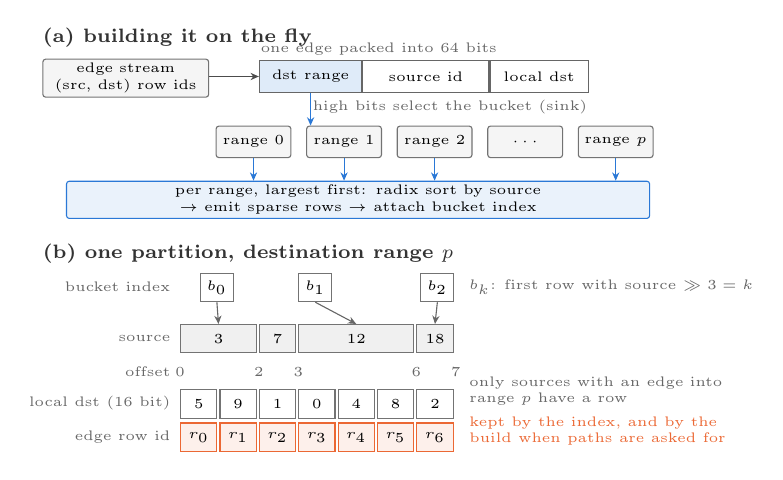
\begin{tikzpicture}[
  font=\tiny,
  >={Stealth[length=3pt,width=2.6pt]},
  box/.style={draw, rounded corners=1pt, align=center, inner sep=1.5pt, minimum height=4mm, anchor=north west},
  data/.style={box, draw=black!55, fill=black!4},
  opstep/.style={box, draw=opblue, fill=opblue!10},
  fld/.style={draw=black!60, minimum height=4mm, inner sep=0pt, anchor=north west, align=center},
  cell/.style={draw=black!55, fill=white, minimum width=4.6mm, minimum height=3.6mm, inner sep=0pt, anchor=north west},
  rid/.style={cell, draw=ixorange, fill=ixorange!10},
  lbl/.style={font=\tiny, text=black!60, inner sep=0.5pt},
  head/.style={font=\scriptsize\bfseries, text=black!80, inner sep=0pt, anchor=north west},
]
% ------------------------------------------------------------------ (a) build on the fly
\node[head] at (0,0) {(a) building it on the fly};
\node[data, text width=2.0cm] (stream) at (0,-0.4) {edge stream\\ (src, dst) row ids};
\node[lbl, anchor=south west] at (2.75,-0.38) {one edge packed into 64 bits};
\node[fld, minimum width=1.3cm, fill=opblue!15] (f1) at (2.75,-0.42) {dst range};
\node[fld, minimum width=1.6cm, fill=white] (f2) at (f1.north east) {source id};
\node[fld, minimum width=1.25cm, fill=white] (f3) at (f2.north east) {local dst};
\draw[->, semithick, black!70] (stream.east |- f1.west) -- (f1.west);
% buckets
\foreach \i/\t in {0/range 0,1/range 1,2/range 2,3/$\cdots$,4/range $p$} {
  \node[data, minimum width=0.95cm] (b\i) at (2.2+\i*1.15,-1.25) {\t};
}
\draw[->, semithick, opblue] (f1.south) -- node[lbl, right, pos=0.45] {high bits select the bucket (sink)} (f1.south |- b1.north);
% tasks take the ranges largest first
\node[opstep, text width=7.3cm] (task) at (0.3,-1.95) {per range, largest first: radix sort by source $\rightarrow$ emit sparse rows $\rightarrow$ attach bucket index};
\foreach \i in {0,1,2,4} {\draw[->, opblue] (b\i.south) -- (b\i.south |- task.north);}

% ------------------------------------------------------------------ (b) one partition
\node[head] at (0,-2.75) {(b) one partition, destination range $p$};
\def\xo{1.75}      % x of the first edge cell
\def\cw{0.5}       % cell pitch
% bucket index above the sources: source >> 3 selects the bucket
\node[lbl, anchor=east] at (\xo-0.1,-3.3) {bucket index};
\foreach \k/\x in {0/0.25,1/1.5,2/3.05} {\node[cell, minimum width=4.2mm] (k\k) at (\xo+\x,-3.12) {$b_\k$};}
\node[lbl, anchor=west] at (\xo+3.65,-3.3) {$b_k$: first row with source $\gg 3 = k$};
% sparse rows: sources spanning their edge groups
\node[lbl, anchor=east] at (\xo-0.1,-3.95) {source};
\foreach \i/\v/\o/\n in {0/3/0/2,1/7/2/1,2/12/3/3,3/18/6/1} {
  \node[cell, minimum width=\n*\cw cm-0.4mm, fill=black!6] (s\i) at (\xo+\o*\cw,-3.77) {\v};
}
\draw[->, black!60] (k0.south) -- (s0.north);
\draw[->, black!60] (k1.south) -- (s2.north);
\draw[->, black!60] (k2.south) -- (s3.north);
\node[lbl, anchor=east] at (\xo-0.1,-4.38) {offset};
\foreach \o in {0,2,3,6,7} {\node[lbl] at (\xo+\o*\cw,-4.38) {\o};}
% edges: 16-bit local destinations and row ids
\node[lbl, anchor=east] at (\xo-0.1,-4.78) {local dst (16 bit)};
\foreach \j/\d in {0/5,1/9,2/1,3/0,4/4,5/8,6/2} {\node[cell] (e\j) at (\xo+\j*\cw,-4.6) {\d};}
\node[lbl, anchor=east] at (\xo-0.1,-5.2) {edge row id};
\foreach \j in {0,...,6} {\node[rid] at (\xo+\j*\cw,-5.02) {$r_{\j}$};}
\node[lbl, anchor=west, align=left] at (\xo+3.65,-4.62) {only sources with an edge into\\ range $p$ have a row};
\node[lbl, anchor=west, align=left] at (\xo+3.65,-5.13) {\textcolor{ixorange}{kept by the index, and by the}\\ \textcolor{ixorange}{build when paths are asked for}};
\end{tikzpicture}

  \caption{The partitioned CSR. (a) The on-the-fly build: the sink packs each edge into 64 bits and the high bits,
  the destination range, select its bucket; tasks take the buckets largest first, sort each by source and emit its
  partition.
  (b) One partition. Rows exist only for sources with an edge into the range; a source's edges are the slice between
  its offset and the next, stored as 16-bit offsets into the range. The bucket index maps the high bits of a source id
  to its first row. The row ids (orange) are what the CSR index adds, and what the build adds when a query asks for
  paths.}
  \label{fig:partitioned-csr}
\end{figure}

We call this layout the \emph{partitioned CSR}. Partitioning the adjacency by destination range so that a traversal
step writes only a cache-sized slice of the frontier is an established idea, known as CSR
segmenting~\cite{zhang2017cagra} and propagation blocking~\cite{beamer2017blocking}, and GraphChi's shards partition
edges by destination interval for the same reason~\cite{kyrola2012graphchi}. What is specific here is that the layout
is produced in one pass from a join stream inside a relational operator, with radix partitioning and no per-vertex
array, and that the same layout is the on-disk format of a transactional index. The operator's build and the index of
Section~\ref{sec:index} share it for a reason. A partition holds every edge into one destination range, so a traversal
step that processes partition $p$ writes only to vertices of range $p$, and the tasks of one level never write the
same vertex. Destinations inside a
partition are 16-bit offsets, half the size of 32-bit ids, and an index epoch stores exactly this layout plus the
row ids. The difference between the two routes for a single pair puts the build at 22, 128 and 264\,ms for the
1.84, 18.7 and 55.7\,M edges of SF10, SF100 and SF300. \todo{The CSR's size in bytes per edge is not measured in the
frozen run; measure it or drop the size claim.}

\subsection{Traversals}
\label{sec:traversals}

The operator has two traversals and a rule that picks one; the multi-source traversal assigns its lanes in one of
two ways. Both traversals run breadth-first over the partitions and both honour the depth bound. They differ in what a
step costs.

\paragraph{Multi-source traversal.} For many pairs we keep \msbfs~\cite{then2014msbfs}. 512 searches share one sweep
over the adjacency, each search owns a bit in three bit-set arrays per vertex (seen, this frontier, next frontier),
and relaxing an edge is a 512-bit \texttt{or}. A lane is either one pair or one source. With a lane per pair, each
input vector of up to 2048 pairs becomes one batch, in the order the vectors arrive, and a batch runs as waves of 512
lanes. With a lane per source, the formulation of Then et al., a wave packs up to 512 distinct sources, each with the
list of destinations its pairs ask for. After every level a lane records the level of the destinations it has newly
reached and drops them from its list, and a lane whose list is empty is masked out of the next frontier, so it stops
spreading. LDBC BI19 at SF300 asks for 2.4\,M pairs from 1.4\,K sources; that is three waves with a lane per source
and 4.6\,K waves with a lane per pair. A wave holds its three bit sets per vertex, 192 bytes at 512 lanes, which is
86\,MB at SF100. The batches of a lane-per-pair query run in worker groups, at most one per thread. When the working sets of
all groups fit a budget of 512\,MiB, all groups start at once and the bit sets stay in cache; otherwise the scheduler
starts 16 groups, doubles their number while the throughput rises by more than a tenth and steps back when it falls by
more than a tenth. A group whose working set is at most a sixteenth of the budget has its own threads; larger groups
pool their tasks, so a group that waits at the end of its level leaves no thread idle. The waves of a lane-per-source
query run side by side, each with its own working set. \todo{They bypass the worker groups and their memory budget:
a query with many waves allocates all their working sets at once. Route them through the scheduler, or say so.}

A level has two phases, an explore phase that relaxes the frontier into the next bit sets and a check phase that folds
the next bit sets into the seen bits. A summary bitmap marks the vertices with a live lane, and a level whose live
vertices are fewer than a sixteenth of all vertices visits only those, through the bucket index. A dense level sweeps
all sparse rows of all partitions and costs the same whether one lane or five hundred are alive. That is a good trade
when hundreds of lanes are alive and a bad one when one is. One pair over the index takes 13\,ms on the lanes against
4\,ms on the single-source traversal at SF10, and 45 against 9\,ms at SF100. \todo{Single runs before rc5; the rerun's
Section 3 microbenchmarks replace them.}

\paragraph{Single-source traversal.} For few sources we run one search per source with a frontier list, in the shape
Ligra~\cite{shun2013ligra} made standard. The frontier is a vector of vertex ids. While it is smaller than a
sixty-fourth of the vertex count, each frontier vertex is looked up in every partition through the bucket index and
its edges are relaxed with a compare-and-swap on a byte per vertex, so a step costs the frontier plus its edges. When
the frontier grows past that bound the step switches to a sweep over the partitions with a per-vertex level stamp
marking the frontier. The search records the destinations its group of pairs asks for and stops as soon as the last
one is reached, or at the depth bound. When the query asks for paths, the traversal also records, per vertex, the
vertex and the edge through which it was first reached, and the result scatter walks that chain backwards
(Section~\ref{sec:paths}). The multi-source traversal cannot afford that; a parent per lane per vertex is 512 times
the memory.

\paragraph{Choosing.} When the pairs are complete, the operator estimates the distinct sources and destinations with
HyperLogLog sketches (64 registers, about 13\% error, enough for a threshold). With at most 16 distinct sources the
single-source traversal runs, one group per source and the threads divided over the groups. With more sources and at
least four pairs per source the multi-source traversal runs with a lane per source, and otherwise with a lane per
pair. Paths and reach always use the single-source traversal, because a path needs a parent per vertex and reach
returns a distance per vertex, and the lanes keep neither. The same sketches decide the orientation. When
there are at least four times as many distinct sources as destinations and reverse partitions are available, which is
the case for an undirected pattern and for an index that stores its reverse side (Section~\ref{sec:index}), the
search starts from the destinations; the on-the-fly build produces forward partitions only. Both rules are
thresholds today, and Section~\ref{sec:strategy} discusses what a cost model needs in order to replace them. The
reverse orientation pays off when many sources share one destination, the shape of LDBC BI20
(Section~\ref{sec:eval-ablation}). \todo{Confirm after the full sweep whether the reverse side stays; then describe it
in Sections 3.2 and 4.} Twenty sources with 200 destinations each, over the index, take 13\,ms on the single-source
traversal, 20\,ms with a lane per source and 86\,ms with a lane per pair at SF10, and 91, 79 and 509\,ms at SF100.
On BI19 at SF300 the lanes per source take 1.6\,s against 30.6\,s for one search per source, and 4.7 against
43.8\,GiB of memory at the peak, because each single-source search keeps a distance, a seen byte and a level stamp
per vertex and 1.4\,K of them run at once. \todo{Single runs before rc5; confirm from the rerun.}

\paragraph{Unbound destinations.} A pattern whose destination carries no condition, every person reachable from $a$,
would produce one candidate pair per vertex. The rewrite recognises this case and asks the operator for the
\emph{reach} of each source instead, one single-source traversal per source that returns every reached vertex with its
distance; the destination table is joined back afterwards only when the query projects its columns. The sources
$\times$ all queries of Section~\ref{sec:eval} run this way.

\paragraph{Pairs with an unknown source or destination.} A pair whose source or destination is \texttt{NULL}, or whose
key is absent from the index, has no path. The operator answers \texttt{NULL} for it without searching and without
changing the traversal chosen for the other pairs of the query. A vertex without edges is searched like any other and
its search ends after one level.

\subsection{Parallelism as a chain of events}
\label{sec:phases}

A BFS level is a parallel sweep followed by a serial decision about which vertices were reached, whether any lane is
still alive and whether the depth bound is hit. The operator runs every traversal as a \emph{chain of per-phase
events}. A phase is a set of tasks that run independently and finish; when the last one finishes, the event's
completion callback runs the serial step once and inserts the event of the next phase. The on-the-fly build has the
same shape with fewer phases. The partitioning happens in the sink as the edges stream in, one event's tasks sort and
emit the ranges, and its completion callback publishes them. Each phase still waits for the one before it, but no task ever blocks its thread waiting for another task. This is the shape
\duckdb's own operators have, and it is what lets the operator share \duckdb's fixed thread pool with other queries.
The scheduler may interleave the tasks of concurrent queries freely, and an error or an interrupt stops the operator
at the next task boundary. The same abstraction covers the multi-source traversal
(two phases per level and batch) and the single-source traversal (one event per level and source group; a group with a
single worker runs all its levels in one task). The cost is one or two events per level, which is microseconds. The
concurrent-reader experiment of Section~\ref{sec:eval} runs 16 readers against one writer at 32 workers per query
with no coordination beyond \duckdb's scheduler.

\subsection{Paths}
\label{sec:paths}

\texttt{element\_id(p)}, \texttt{vertices(p)} and \texttt{edges(p)} are answered by the same operator in a second
mode that returns, per pair, the list $[v_0, e_0, v_1, \dots, v_k]$ of vertices and edge row ids. The vertices are
row ids when the CSR is built in the query and keys when it is read from an index. The
single-source traversal records parents as described above; the scatter walks from the destination to the source,
maps vertex ids to row ids or keys and edge positions to row ids, and reverses the list. \texttt{path\_length(p)} is then
$\lfloor\text{len}/2\rfloor$, and \texttt{vertices} and \texttt{edges} are the even and odd positions, which is also
how the SQL fallback of \duckpgq defines them, so the build route and the fallback return the same lists. Edge row ids are available because
the build keeps one per edge position when paths are requested and the index keeps them always
(Section~\ref{sec:index}), so a path can be joined back to the edge table for its properties. Paths cost more than
lengths when the pairs have many sources, because paths need the single-source traversal and lengths use the lanes.
For 2048 random pairs over the index, paths take 3.6 times as long as lengths at SF10 and 4.5 times at SF100.
\todo{Single runs before rc5; confirm from the rerun.}

\section{An MVCC-Consistent CSR Index}
\label{sec:index}

\todo{2.5 pages. Figure: epoch + change log + per-reader snapshot.}
\subsection{Design constraints from the extension interface}
\todo{What the index type interface delivers (appends, deletes with row ids, serialize, WAL replay) and what it does
not (commit ids, visibility); keys not row ids identify vertices; the index may not evaluate visibility at past
bounds because the engine garbage-collects row versions.}
\subsection{Epochs, change groups and snapshots}
\todo{Immutable epoch CSR with dictionary and row ids per position; change log stamped per commit group; a reader
decides visibility once per group with CanFetch; snapshot = epoch partitions + delta partitions + suppressed bitmap;
private snapshot for writing transactions; snapshot cache keyed by (generation, newest visible group).}
\subsection{Fold}
\todo{Rebuilding an epoch from a live transaction, generation stamping, retained epochs, id re-resolution; fold
ratio policy.}
\subsection{Checkpoint, recovery and parallel load}
\todo{Segments in the index allocator, manifest in storage options, WAL replay through Append/Delete, parallel
deserialization numbers (SF300 1.15 s to 0.09 s).}
\subsection{Path reconstruction}
\todo{Parent pointers in the single-source traversal, edge row ids from epoch and delta partitions, keys for vertices;
what the multi-source traversal cannot do and why.}
\subsection{Correctness}
\todo{Argument: a reader sees exactly the edges whose rows are visible to its transaction; cases: concurrent insert,
delete of an epoch edge, delete of a delta edge, rollback, fold during a long snapshot, restart.}

\section{Choosing a Strategy}
\label{sec:strategy}

\todo{1 page. Build per query vs index; multi-source traversal vs single-source traversal; forward vs reverse; the statistics the
operator has (pair count, distinct sources/destinations via HLL, edge count, pending change-log size) and the cost
model calibrated from the sweeps (W13). The engine hooks an extension needs for this and which ones are missing.}

\section{Evaluation}
\label{sec:eval}

\todo{3 pages. Setup: m7a.8xlarge (32 cores, 128 GiB, gp3 1000 MB/s), DuckDB v2.0 at commit X, Kuzu 0.11.3, Neo4j Y,
Memgraph, FalkorDB; LDBC SNB SF1-SF300 knows graph, Graphalytics sets; query shapes point-to-point (1024 pairs),
single-source (sssp), all-pairs blocks, Graphalytics BFS; cold = fresh process, warm = second query.}
\subsection{Read-only: build per query vs index vs native systems}
\todo{Table: per SF and query shape, operator / index cold / index warm / Kuzu / Neo4j. SF300 warm 32 threads: sssp
0.30 / 0.17 / 0.031 s; point-to-point 1.61 / 1.11 / 0.96 s. Index load 0.09 s at 32 threads.}
\subsection{Updates}
\todo{LDBC BI insert/delete batches; sequential and concurrent (1 writer, 1-16 readers); index with and without fold vs
build per query vs Kuzu/Memgraph/FalkorDB; query latency over pending operations; update cost per commit.}
\subsection{End-to-end queries}
\todo{LDBC IC13, IC14 (paths), BI19/20 on all systems (W17).}
\subsection{Ablations}
\todo{Kernels (lanes vs per-source, hybrid expansion, bucket index), orientation, grouping, phased events vs barriers,
fold ratio, snapshot cache; thread scaling 1-32; memory per edge during build and for the index.}

\section{Related Work}
\label{sec:related}

% Draft 22 Oct 2026. Citations marked \cn or with VERIFY comments in references.bib still need checking.

\paragraph{Graph queries in relational engines.}
Making a relational engine answer graph queries has a long history: as a rewrite of pattern matching into joins
over edge tables~\cite{sun2015sqlgraph,jindal2014vertexica,fan2015grail}, as a query language layered on an
RDBMS~\cite{vanrest2016pgql}, and most recently through \sqlpgq, the graph pattern matching part of the SQL
standard~\cite{deutsch2022gql}. \duckpgq~\cite{tenwolde2023duckpgq} implements \sqlpgq as a \duckdb extension that
rewrites \texttt{MATCH} into relational SQL; this paper extends it with a physical operator and an index while
keeping the extension boundary. Systems that modify the engine for graph workloads add predefined joins and
adjacency structures (GRainDB~\cite{jin2022graindb,jin2022predefinedjoins}), worst-case optimal joins for cyclic
patterns (EmptyHeaded~\cite{aberger2017emptyheaded}, Umbra~\cite{freitag2020wcoj}), or compressed adjacency
indexes for aggregation-heavy queries (GQ-Fast~\cite{lin2016gqfast}). Their adjacency structures are built inside
the engine and share its storage and transaction code; ours is a derived structure that an extension maintains
through the public index interface, which is what forces the snapshot design of Section~\ref{sec:index}.

\paragraph{Path finding.}
Variable-length and shortest-path patterns are the part of \sqlpgq that relational operators serve worst.
Recursive common table expressions evaluate them as iterated joins with a frontier table per step, and both
RaSQL~\cite{gu2019rasql} and the Umbra work on recursive SQL~\cite{hirn2019recursion} optimize that evaluation
rather than replace it. Our operator instead runs a graph traversal over a compressed sparse row (CSR) layout, in the
tradition of Grail~\cite{fan2015grail} and of in-database BFS kernels~\cite{jindal2014vertexica}. The kernel is
multi-source BFS~\cite{then2014msbfs}, which shares one sweep over the adjacency among 512 concurrent searches held
in bit sets; direction-optimizing BFS~\cite{beamer2012direction} supplies the push/pull variant we compare against,
and frontier-list BFS as in Ligra~\cite{shun2013ligra} is the shape of our per-source kernel for point queries. The
GraphBLAS~\cite{davis2019graphblas} expresses the same traversals as sparse matrix products; RedisGraph and its
successor FalkorDB build a graph database on it~\cite{cailliau2019redisgraph}.

\paragraph{Native graph database systems.}
Neo4j, Kuzu~\cite{feng2023kuzu}, TigerGraph~\cite{deutsch2019tigergraph} and Memgraph keep adjacency lists as
their primary storage, so a shortest path never needs a structure to be built; the price is a separate system next
to the relational data. Kuzu is the closest design point to ours: columnar storage, vectorized execution, and
factorized intermediate results, with recursive joins for variable-length patterns~\cite{feng2023kuzu}. Our
evaluation uses Kuzu and Neo4j as the native baselines and shows that a relational engine with the index closes the
gap on read-only point and single-source queries while keeping updates in the same transaction as the tables.

\paragraph{Dynamic and versioned graph structures.}
Updating a CSR is the classic weakness of the layout, and a line of work replaces it with structures that absorb
edge updates: packed memory arrays and compressed sparse formats with gaps~\cite{wheatman2018pcsr,deleo2021teseo},
sorted blocked adjacency lists~\cite{fuchs2022sortledton}, log-structured snapshots~\cite{macko2015llama}, and
purely functional trees that give every reader its own version~\cite{dhulipala2019aspen}. LiveGraph~\cite{zhu2020livegraph}
and Teseo~\cite{deleo2021teseo} offer transactional semantics with multi-version concurrency over such structures,
and Sortledton~\cite{fuchs2022sortledton} shows the cost of versioning inside the structure itself. These systems
own both the graph and its transaction manager. Our index does not: visibility is decided by the host engine's
row versions, and the index stores an immutable CSR per epoch plus a change log stamped per commit group, which is
closer to how an RDBMS maintains a materialized view than to a dynamic graph structure. Surveys of the dynamic graph
literature~\cite{besta2023dynamic} and the experimental comparison of these structures~\cite{deleo2019pma} cover the
design space.

\paragraph{Indexes under MVCC.}
Relational indexes under multi-version concurrency either store version information per entry or, as in
PostgreSQL and \duckdb's ART~\cite{leis2013art}, keep only row identifiers and consult the row's versions on every
probe~\cite{wu2017mvcc,neumann2015mvcc}. A traversal that touches millions of edges cannot afford a version check
per edge, which is why the index of Section~\ref{sec:index} checks visibility once per commit group and serves a
whole BFS from one immutable snapshot. The extension builds on the index type interface that \duckdb exposes to
extensions~\cite{duckdb2019}, the same hook that its spatial index uses; to our knowledge this is the first use of such
an interface for a snapshot-consistent graph structure.

\section{Conclusion}
\label{sec:conclusion}

% Written 29 Oct 2026 from the rc1 numbers.

The CIDR version of \duckpgq answered shortest-path queries with UDFs, and the UDFs inherited \duckdb's
tuple-driven parallelism, so a query with few pairs ran on one core and every query rebuilt the CSR. This paper
removed both limits without leaving the extension. The path-finding operator takes its parallelism from a CSR
partitioned by destination range and runs every traversal as a chain of events in \duckdb's scheduler. The CSR index
keeps the graph across queries and stays consistent with \duckdb's MVCC through epochs and a change log whose
visibility \duckdb itself decides, once per change group. Because the operator answers many pairs with one
traversal, the gap to the native graph systems grows with the number of pairs. At SF100 one query for 65\,536 pairs
takes 3.5\,s, against 155\,s for Neo4j and 169\,s for Kuzu, and at SF300 it takes 10\,s while every other system
exceeds ten minutes. Under the LDBC update stream a commit costs 15\,ms, against 342\,ms for Kuzu, and every
transaction sees exactly the edges it may see. \todo{Confirm the numbers against rc2.}

\duckdb's extension interfaces were enough, and where they fell short the gaps are specific. An index callback does
not say which transaction or commit made a change, and nothing can ask about visibility in the past. The scheduler has
no tasks for index work, so a fold runs in the transaction that triggers it. An extension operator can report a
cardinality but not a cost. Each gap cost us a mechanism in this paper, and each would be small to close in the
host system.

In the future, we will replace the thresholds of Section~\ref{sec:cost} with a cost model calibrated on these runs,
move the fold into the background, and extend the operator to weighted shortest paths, to an index over several edge
tables of one property graph, and to path reconstruction in the multi-source traversal.


%\begin{acks}
%\end{acks}

\bibliographystyle{ACM-Reference-Format}
\bibliography{references}

\end{document}
